\documentclass[a4paper, 11pt, french]{report}
\usepackage[utf8]{inputenc}										% package désignant l'encodage
\usepackage[T1]{fontenc}	  									% je sais pas à quoi il sert
\usepackage[francais]{babel} 
\usepackage[colorlinks=true, urlcolor=blue, linkcolor=blue]{hyperref}
\usepackage{graphicx}
\usepackage{wrapfig}
\usepackage{multicol}

\author{Boncorps Robin \& Daniel Gwendal}
\title{Rapport de projet - FTP pair à pair}

\begin{document}
\maketitle

\chapter{Introduction} % lol
Dans le cadre de nos TP de réseaux, nous avons du développer une application client/serveur. Le but de ce projet est de comprendre les principes de fonctionnement des sockets, bases de toutes applications réseaux réparties. C'est dans cette optique que nous avons choisi de développer une application d'échange de fichiers en pair à pair. Nous allons donc, dans le présent rapport, présenter les différents protocoles et moyens utilisés pour mener à bien ce projet. Nous nous intereserons, par la suite, à la modélisation de l'application pour finir par présenter les différentes performances de l'application.

\chapter{Analyse}
Dans cette partie, nous allons présenter succintement les différentes bases sur lesquelles s'appuie l'application.

	\section{FTP : File Transfer Protocol} %robin
	FTP ou File Transfert Protocol est un protocol de communication destiné à l'échange de fichiers sur un réseau TCP/IP.
	FTP obéit à un modéle client-serveur, un client interrogant un serveur distant qui fonctionne sur la machine distante.
	
	
	
	\section{Pair à pair} % gwendal
	\section{Application} % gwendal

\chapter{Modélisation}
	\section{Architecture} %gwendal
	\section{PXP : Personal eXchange Protocol} %robin
		L'application permet d'échanger des fichiers grâce à son propre protocole (de la meme famille que ftp). 
		Ce protocole, que nous nommerons par la suite PXP pour Personal eXchange Protocol, permet le découpage/reconstruction d'un fichier entre 2 machines distante.
	
		\subsection{La trame PXP}
			\begin{figure}[!h]
				\centering
				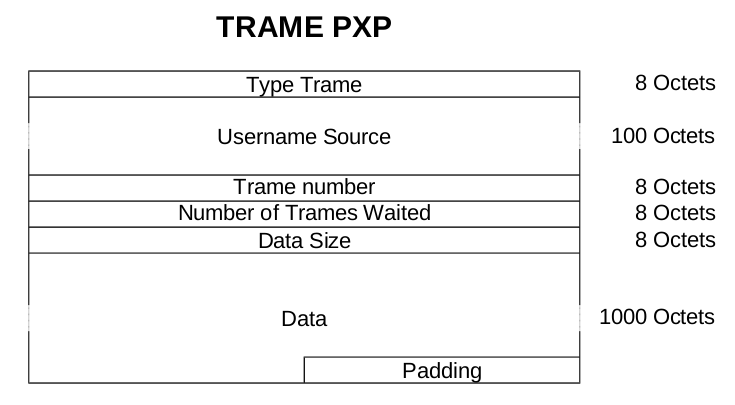
\includegraphics[scale=0.5]{TramePXP.png}
				\label{Trame PXP}
			\end{figure}
			% mettre TramePXP.png
			Signification des champs :
			\begin{itemize}
				\item Type Trame : Le type de trame envoyé (nous détaillerons par la suite les différents types)
				\item Username Source : le nom de l'utilisateur qui envoi la trame
				\item Trame number : le numéro de la trame envoyée
				\item Number of Trame Waited : le nombre de trames attendues pour avoir tout le fichier
				\item Data Size : la taille effective des données comprises dans la partie Data
				\item Data : les données (une partie du fichier)
				\item Padding : 0 ajoutés pour remplir le champ Data
			\end{itemize}
			
			\subsubsection{Type Trame}
				Chaque action effectuée sur une machine distante a un type particulier
				\begin{itemize}
					\item CON\_SERV : demande de connexion au server
					\item ACK\_CON : le serveur accepte votre connexion
					\item DEM\_AMI : demande d'ami pour echange pair à pair
					\item DEM\_CON\_AMI : demande d'établissement d'une connexion avec autre client distant
					\item CHECK\_CON : vérification que le client distant est connecté
					\item CMD\_CON : initialisation du mode commande 
					\item CMD\_HOME : le path home du client distant est envoyé
					\item CMD : envoi d'une commande
					\item LS\_RET : retour d'une commande LS
					\item CD\_RET : retour d'une commande CD
					\item MAJ\_PATH : mise à jour du path courant
					\item CMD\_END : fin du mode commande
					\item DEM\_FIC : demande d'envoi d'un fichier
					\item ENV\_FIC : envoi du fichier
					\item ACK : acquittement de reception du fichier
					\item FIN\_CON\_AMI : fin de connection avec le client distant
					\item FIN\_CON\_SERV : fin de connexion avec le serveur
					\item ERROR : Trame d'erreur sur le client distant
				\end{itemize}
			
			
		\subsection{Transfert de données}
			Lors de l'envoi d'un fichier, si sa taille dépasse la taille maximum des datas d'une trame (1000 Octets ici), le fichier doit être découpé en plusieurs partie. 
			Ceci se fait tout simplement en parcourant le fichier par bloc de 1000 octets et en envoyant directement une trame contenant ces données.
			Il faut toute fois noter qu'il faut tout d'abord connaître la taille du fichier pour déterminer le nombre de trames qui vont être envoyées.
			On determine donc le nombre de trame a envoyer ainsi que la taille des données qui seront contenues dans la dernière trame (qui peut ne pas être complete)
			
			
			La reconstruction du fichier par ecriture direct des données contenues dans les trames reçues dans le fichier destination. Lors de la reception de la première trame du fichier, le nombre de trame attendu est extrait et permet de savoir combien de trame sont encore à recevoir. 
			Toutefois, la reception des trames du fichier s'arretera si l'ordre n'est pas respecté. Ceci n'est pas sensé arriver car TCP gère déjà l'ordre d'arrivé des trames avec son propre système.
			
\chapter{Résultats}
	\section{Vitesses de transfert}  %gwendal
	\section{Format de trames} %robin
	Nous avons opté pour une taille de trame de 1132 octets (entête comprise) pour ne pas dépasser la taille maximale des données d'une segment de TCP qui est 1500 octets. Ceci permet de ne pas avoir a redécouper les données envoyées, ce qui ralentirait la vitesse de transfert.
	

\chapter{Conclusion}
	\section{Apports} %gwendal
	\section{Difficultés rencontrées} %robin
	Nous avons principalement rencontré des difficultés lors du découpage des fichiers ainsi qu'au niveau de la procedure de reception de trame. 
	La première difficulté était de savoir comment découper un fichier et de le reconstruire après.
	La deuxième difficulté était que, lors de la reception de toutes les trames contenant le fichier, le système s'arrêtait. Ce problème était du à l'utilisation de la fonction read dans un socket pour récupérer son contenu. En effet, cette fonction n'attend pas que le buffer de reception soit rempli, ce qui entrainait une perte d'information. La solution apporté a été d'utiliser la fonction recv qui permet, grâce à un flag, d'attendre que le buffer soit rempli avant de recevoir une autre trame. 
\end{document}
